\subsection{概要}
	前章ではある地域の実際の要望をシステムによって実現した.
	今後システムを発展させるには2章1節で述べたような
	様々な電子化された医療情報を入力データとして
	受けつける必要がある.
	これを実現するためにNoSQLデータベースのCouchDBを用いて
	システムを開発する.

\subsection{CouchDBのドキュメントの構造}
	本研究ではひとつの医療行為に対してひとつのドキュメントで管理する.
  本研究で使用するドキュメントが保持する情報を表\ref{tab:doc}に示す.
  これに従ってJSONで記述された医療情報の内容を図\ref{json-for-doc}に示す.
  CouchDBのドキュメントとして必須の項目である\_id,\_rev以外にdata要素だけを用意した.
  今後,必要になったときに他の要素を追記することは可能である.

	\begin{table}[htb]
    \begin{center}
      \caption{ドキュメントが保持する情報}
      \begin{tabular}{|l|c|r|r|}\hline
      Key & Value \\ \hline \hline
      \_id &  患者名、ドキュメント作成日をドキュメントIDとしている. \\ \hline
      \_rev & \shortstack{ドキュメントの更新回数を示す. \\ 更新時に参照し競合を防ぐ.} \\ \hline
      %name & 患者の名前 \\ \hline
      data & \shortstack{医療行為によって得られた情報を格納.} \\ \hline
      \end{tabular}
      \label{tab:doc}
    \end{center}
  \end{table}

  \begin{figure}[htbp]
    \begin{center}
      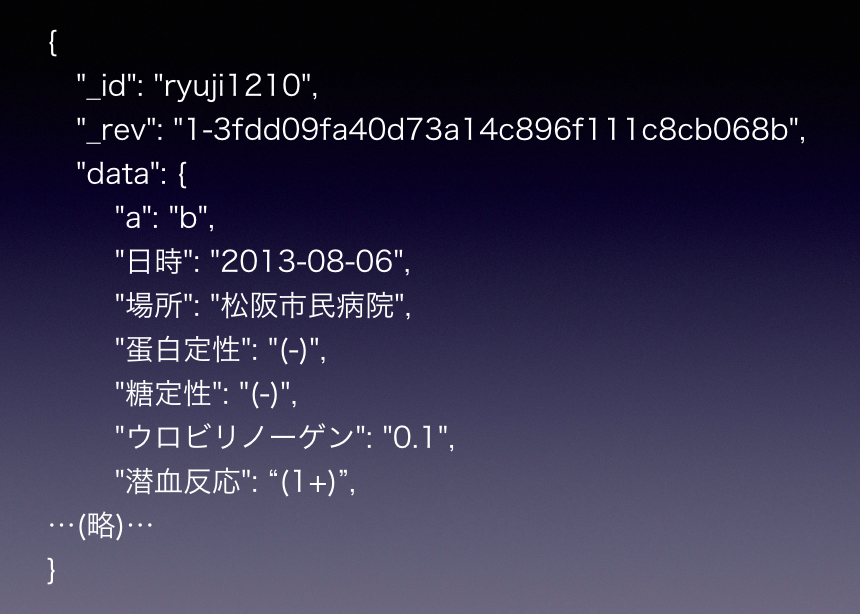
\includegraphics[width=10cm, bb=0 0 1027 737]{./gazou/json-for-doc2.png}
    \end{center}
    \caption{ドキュメントのJSONの構造}
    \label{json-for-doc}
  \end{figure}





\subsection{実装}
	開発にはJavascriptのフレームワークであるNode.jsを用いた.
	また,データベースにはCouchDBを用いた.
	その他,使用したライブラリ群は付録に記載する.\cite{bibi9}

	\subsubsection{同義キーを活用したデータ閲覧}

		ユーザはログイン後検索ワードを送信すると,
		CouchDBのドキュメントのdataオブジェクトに検索ワードを
		含でいたキーと値の組を列挙する.
		データの読み取り方はドキュメント名:項目名→値となっている.

		図\ref{getdb}は白血球という単語で検索した結果である.
		検索結果のドキュメント名の日付が前後しているが,
		これはデータを入力したときの日付であるため,
		日付の順序は意味を持ってはいない.

			\begin{figure}[htbp]
				\begin{center}
					%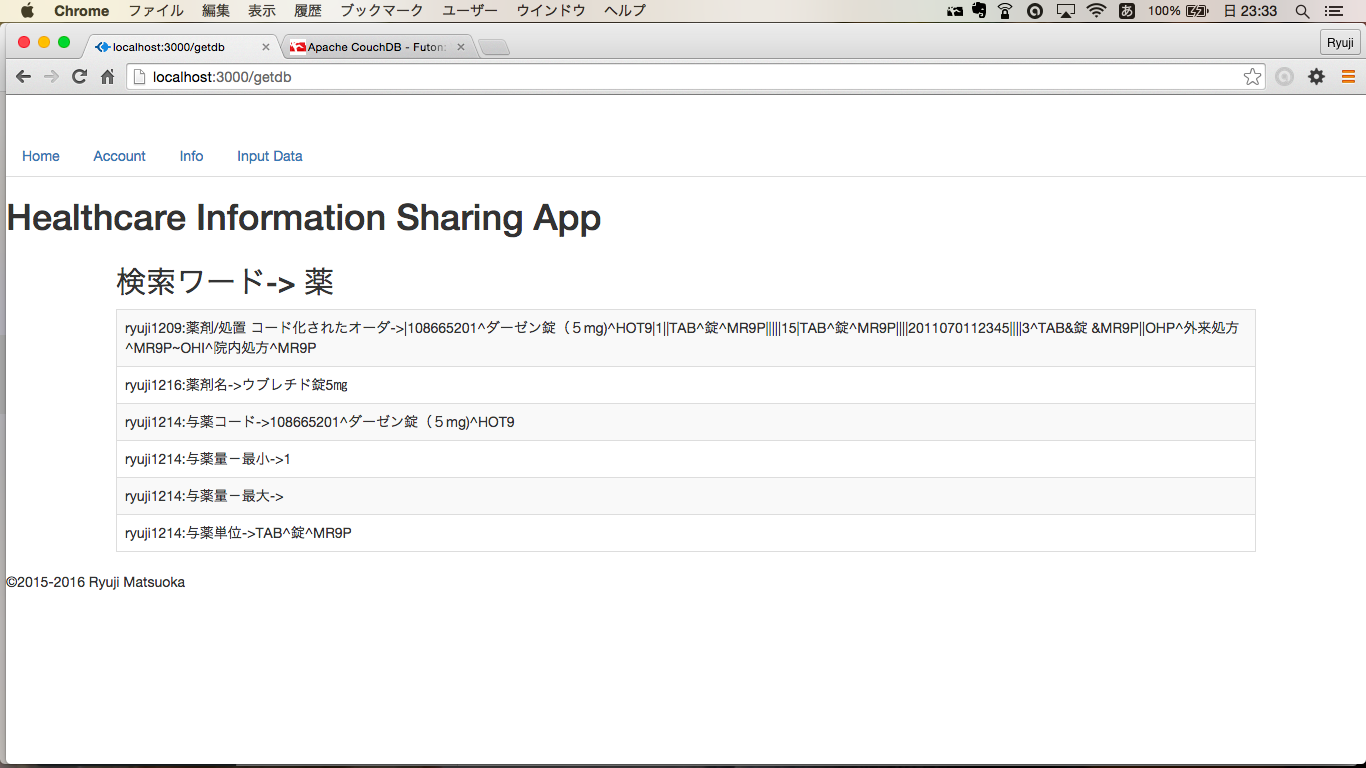
\includegraphics[width=15cm, bb=0 0 1366 1078, clip]{./gazou/getdb.png}
					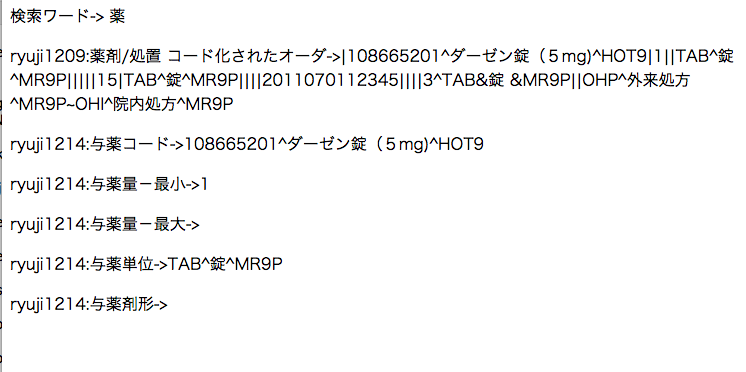
\includegraphics[width=15cm, bb=0 0 652 603, clip]{./gazou/getdb2.png}
				\end{center}
				\caption{白血球で検索した様子}
				\label{getdb}
			\end{figure}


		図\ref{relation}は投薬データの処方日と診断データの日時が同義として
		登録されている様子を示している.
		図\ref{relationApp}は検索ワードを処方としたときの結果を示しており,
		処方をキーに含むデータが検索結果として表示される.
		さらに,検索結果に処方日があり,これは日時と同義として登録されているため,
		日時のデータも検索結果として表示される.


		\begin{figure}[htbp]
			\begin{center}
				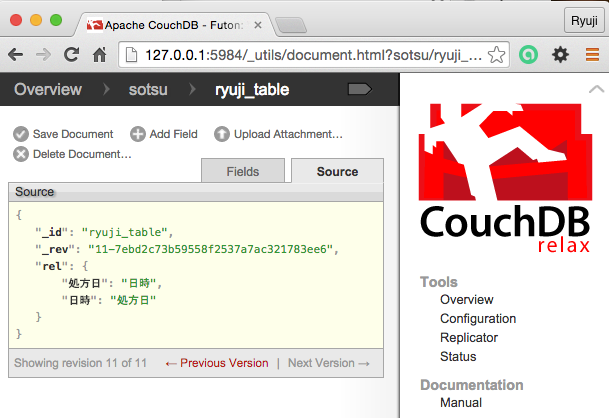
\includegraphics[width=10cm, bb=0 0 609 478, clip]{./gazou/relation2.png}
			\end{center}
			\caption{同義キーを管理するドキュメント}
			\label{relation}
		\end{figure}

		\begin{figure}[htbp]
			\begin{center}
				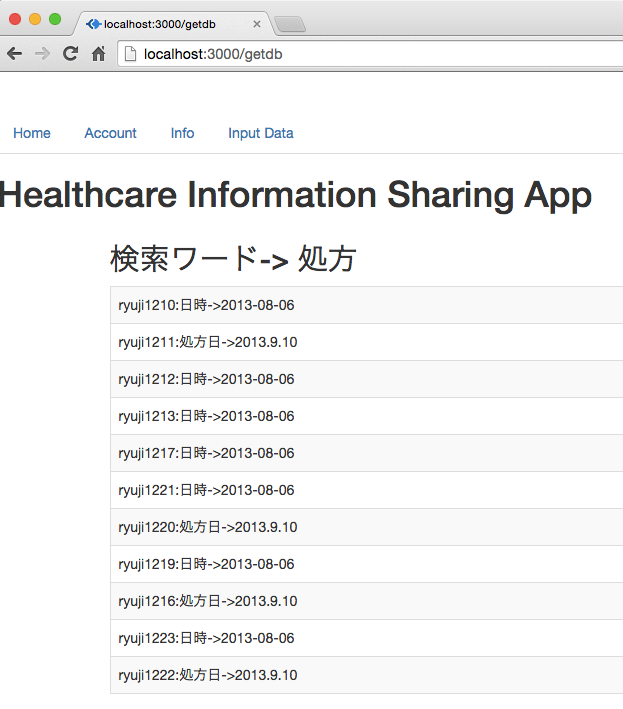
\includegraphics[width=15cm, bb=0 0 609 528, clip]{./gazou/relationApp4.png}
			\end{center}
			\caption{処方と検索して同義キーとして登録されている日時も表示する}
			\label{relationApp}
		\end{figure}



		\subsubsection{CSVファイルの整形}

			\begin{figure}[htbp]
				%\begin{center}
					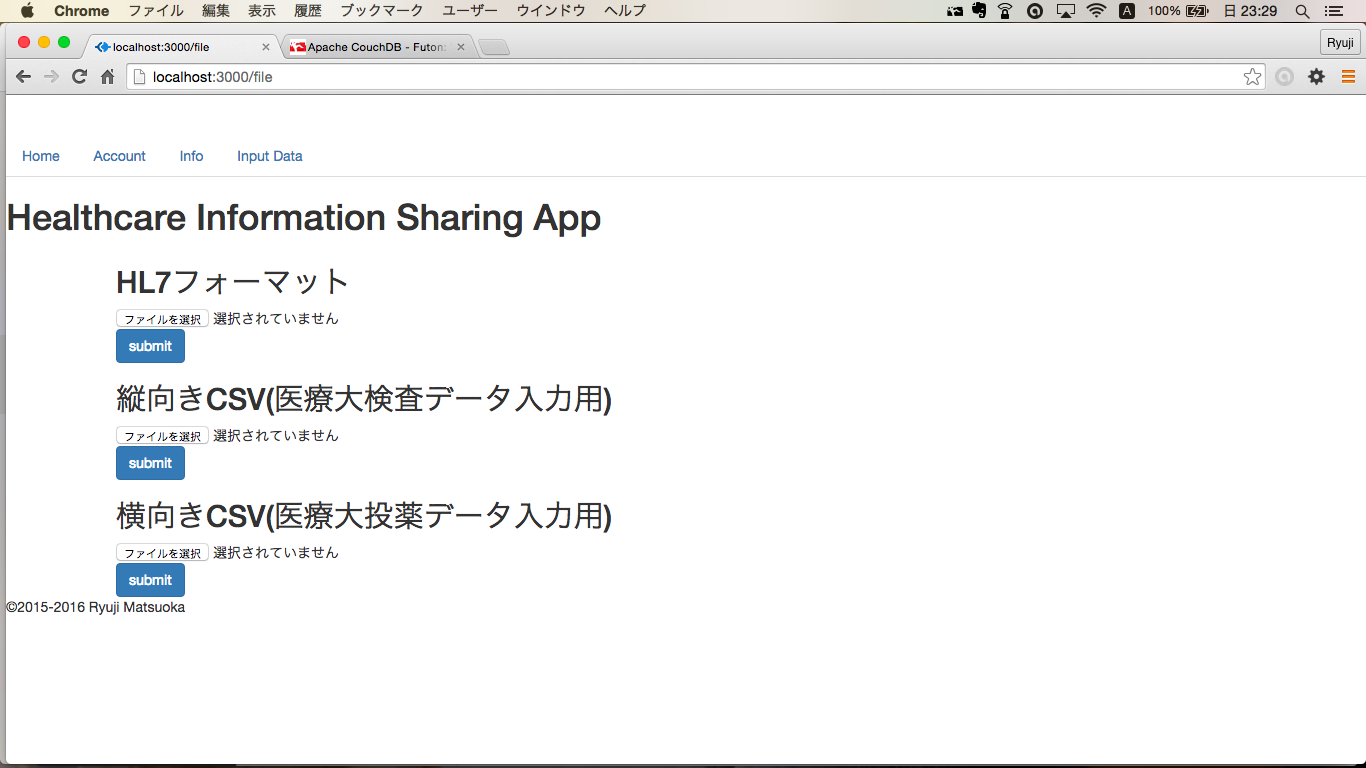
\includegraphics[width=15cm, bb=0 0 1366 1078, clip]{./gazou/fileiopage.png}
				%\end{center}
				\caption{ファイル入力ページ}
				\label{fileiopage}
			\end{figure}
			ファイル入力はユーザがログイン後,図\ref{fileiopage}の画面で行う.
			CSVファイルは入力ファイルの行,列のどちらかに医療情報,
			他方に日付をとっているものを想定している.
			このため,CSV入力ファイルに複数回の診療の記録があることを許容する設計にしており,
			行ごとに,または列ごとに1つのドキュメントを
			生成することで,1度の診療で1つのドキュメントとしている.
			図\ref{csv-data-trans}は入力内容とCouchDBへの登録内容の
			対応を表したものである.
			列ごとに検査データが記入されているエクセルファイルの
			項目が記入された列と一回の検査データを表したものが
			図中左の表である.
			これを項目と検査データの組にして,
			CouchDBのdata要素として入力する.
			同様の処理を以降の検査データの列に対しても行う.

			これによって入力された検査データが図\ref{iryoudai-kensa-data}
			である.
			また,行に項目を取っている投薬データを入力したものが
			図\ref{iryoudai-touyaku-data}である.
			さらに,患者からの入力を想定した家庭用血圧計の
			出力CSVファイルが図\ref{blood-data}であり,
			これをCouchDBに入力したものが図\ref{blood-data-couch}である.


			\begin{figure}[htbp]
				\begin{center}
					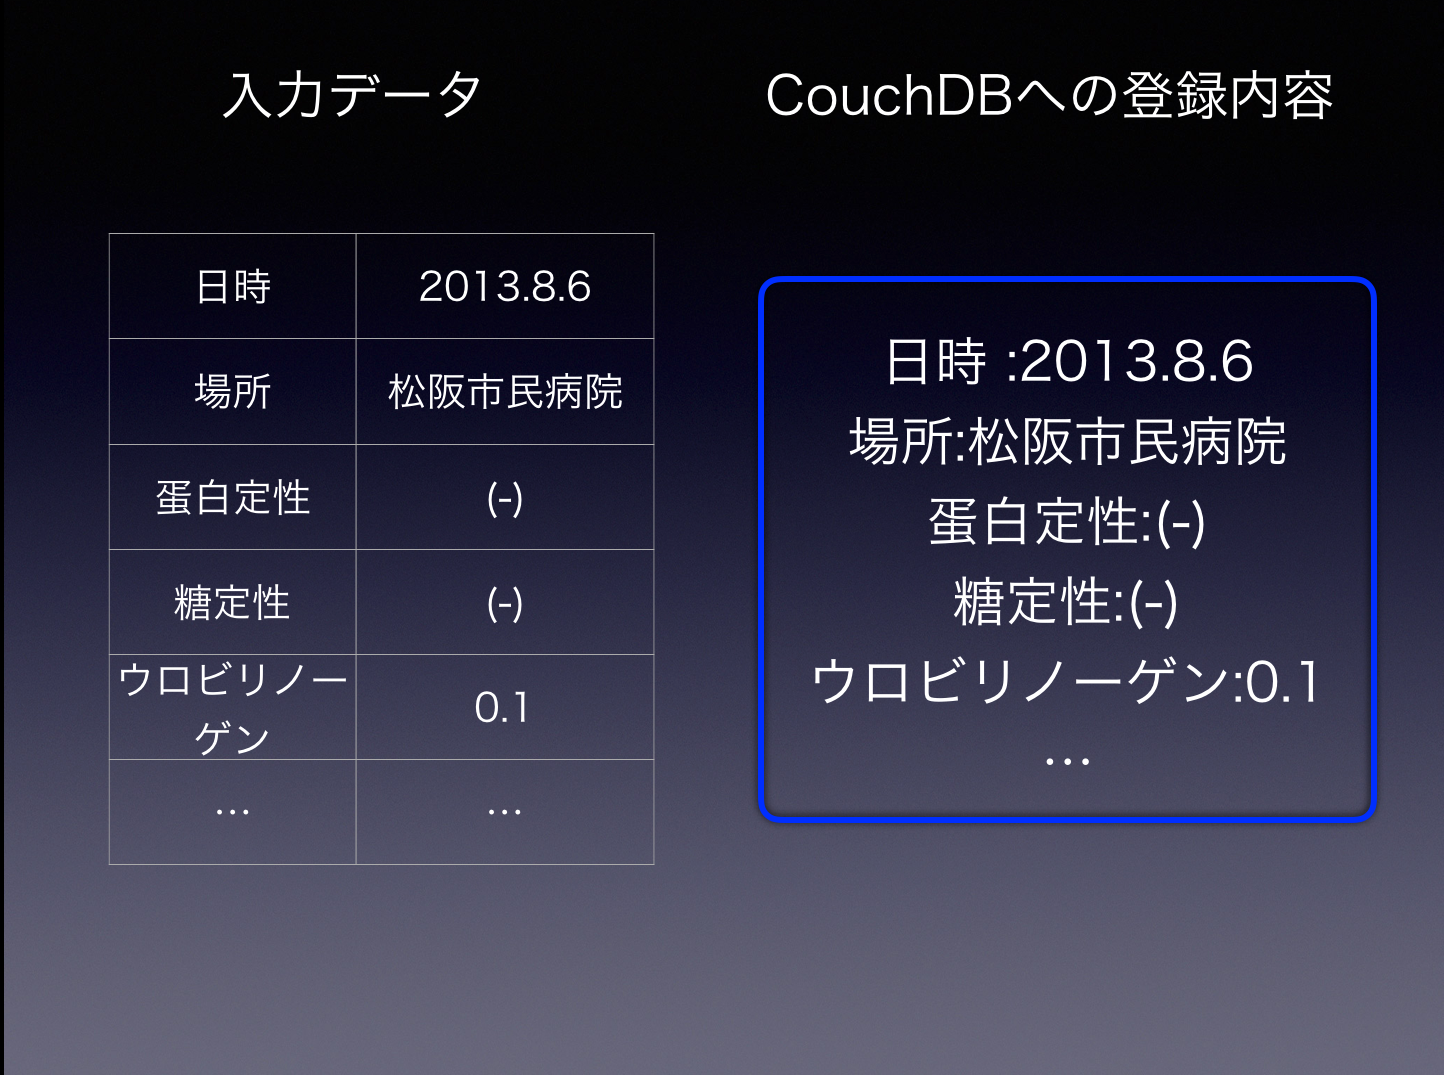
\includegraphics[width=15cm, bb=0 0 1435 1073, clip]{./gazou/csv-data-trans2.png}
				\end{center}
				\caption{入力内容とDB登録内容の対応}
				\label{csv-data-trans}
			\end{figure}

			\begin{figure}[htbp]
				\begin{center}
					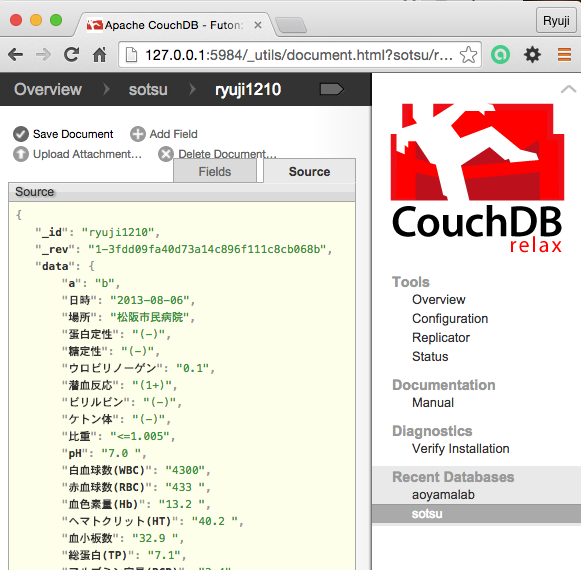
\includegraphics[width=10cm, bb=0 0 581 571, clip]{./gazou/kensa-data.png}
				\end{center}
				\caption{CouchDBに投入された医療大の検査データ}
				\label{iryoudai-kensa-data}
			\end{figure}


			\begin{figure}[htbp]
				\begin{center}
					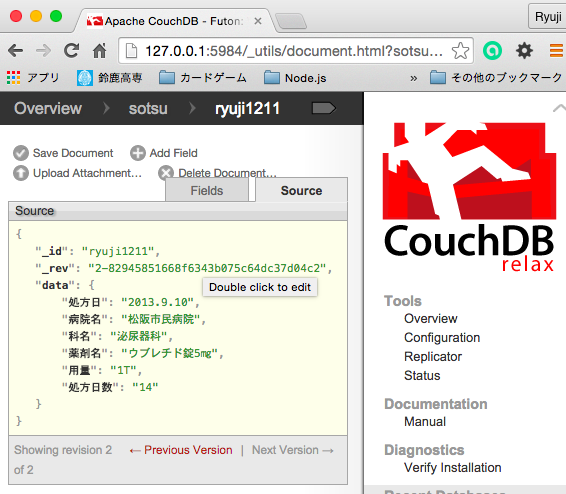
\includegraphics[width=10cm, bb=0 0 576 573]{./gazou/touyaku-data2.png}
				\end{center}
				\caption{CouchDBに投入された医療大の投薬データ}
				\label{iryoudai-touyaku-data}
			\end{figure}

			\begin{figure}[htbp]
				\begin{center}
					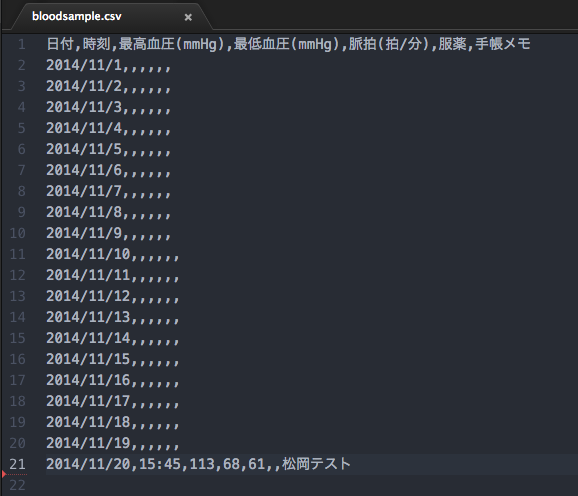
\includegraphics[width=10cm, bb=0 0 578 469]{./gazou/blood-data.png}
				\end{center}
				\caption{家庭用血圧計の出力データ}
				\label{blood-data}
			\end{figure}

			\begin{figure}[htbp]
				\begin{center}
					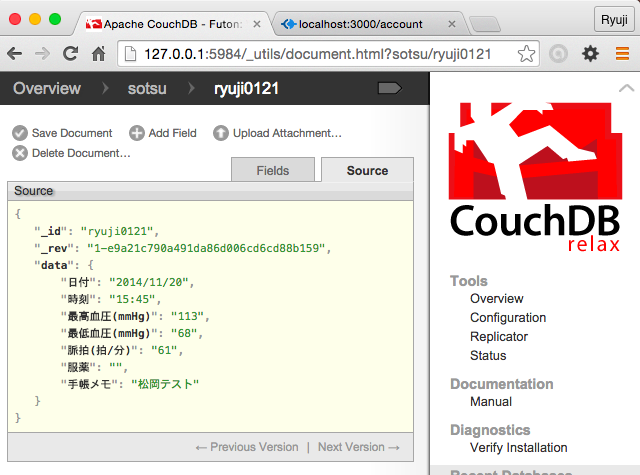
\includegraphics[width=10cm, bb=0 0 640 475]{./gazou/blood-data-couch.png}
				\end{center}
				\caption{CouchDBに入力された家庭用血圧計の出力データ}
				\label{blood-data-couch}
			\end{figure}

		\subsubsection{HL7ファイルの整形}
			ファイル入力方法はCSVファイルの場合と同様である.
			前述のHL7のデータ定義に基づいて入力ファイルからデータを格納していく.
			HL7の出力ファイルはパイプ区切りで記述されており,
			並び順にデータの意味が割り振られている.
			図\ref{hl7-data-trans}の枠内のデータがOBX-3という
			セグメントのデータである.
			このセグメントの意味をアプリケーション内のテーブルから参照し,
			意味とデータをJSON形式に整形してCouchDBに登録する.


			本研究では前述のCSVファイルのような医療規格にのっとっていない医療情報との関連付けを課題としている.
			そこでHL7にのっとったファイルからデータを抜き出し,
			データの配置によって割り振られている意味をキーとしてデータベースに
			格納していく.

			\begin{figure}[htbp]
				\begin{center}
					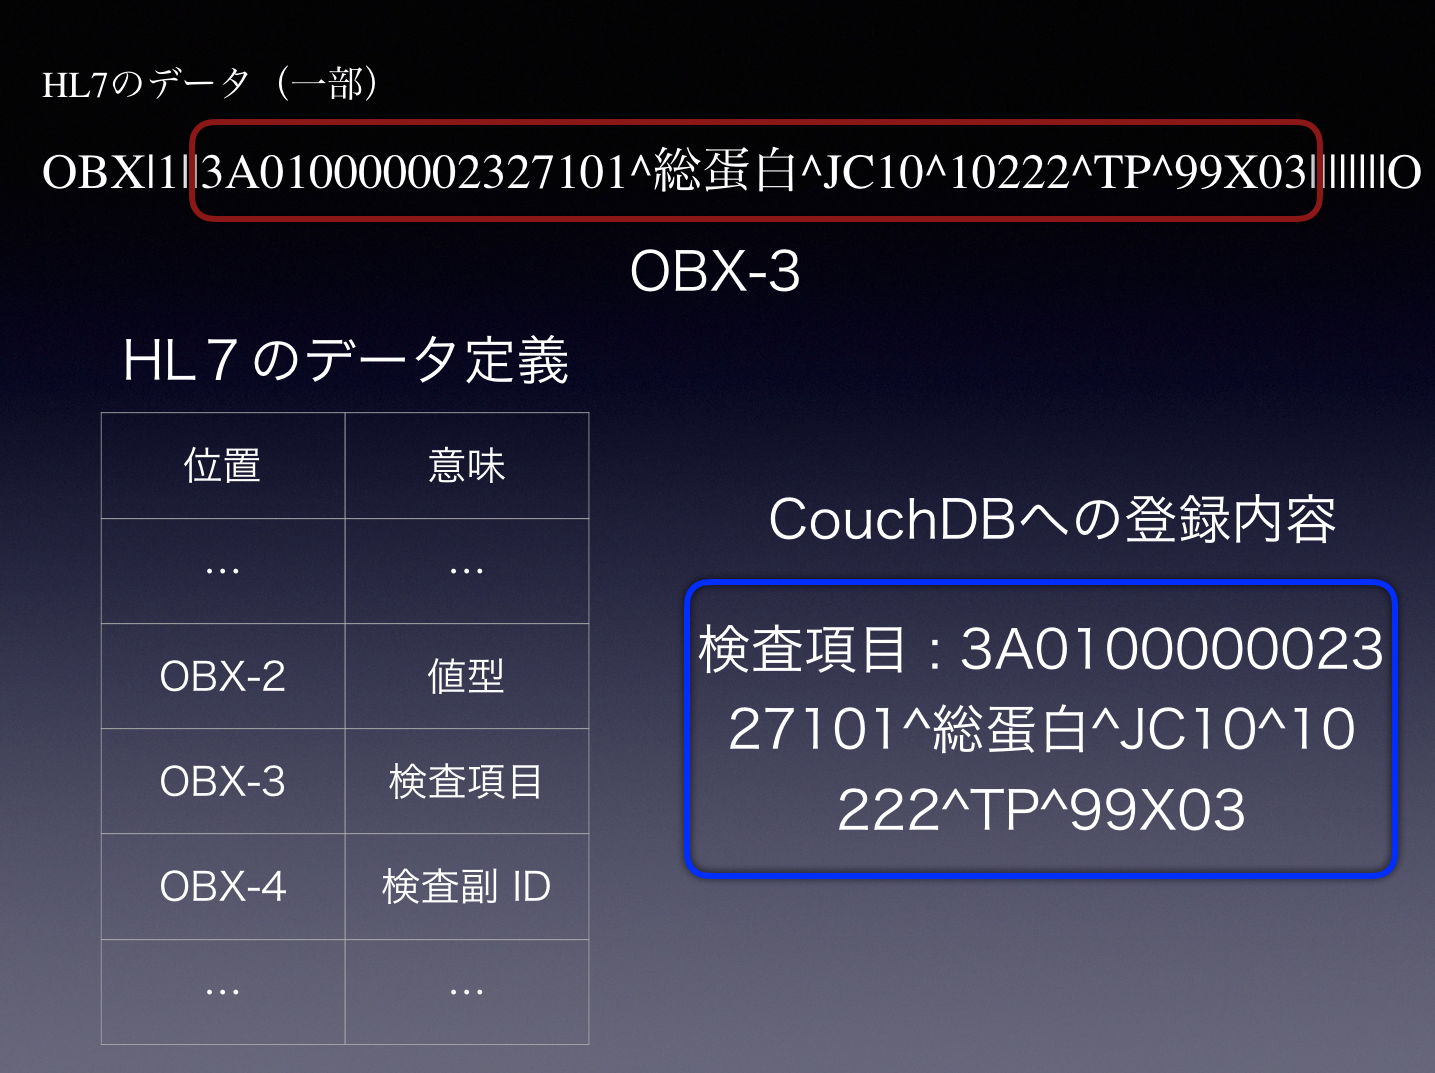
\includegraphics[width=15cm, bb=0 0 1435 1073]{./gazou/hl7-data-trans2.png}
				\end{center}
				\caption{HL7の生データからJSONへの変化}
				\label{hl7-data-trans}
			\end{figure}

			\begin{figure}[htbp]
				\begin{center}
					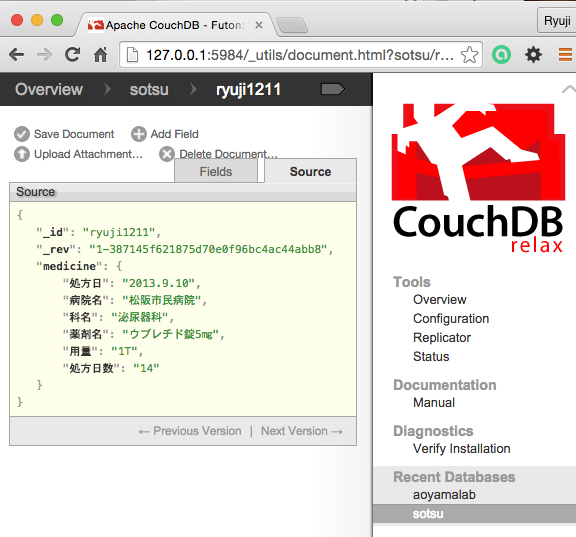
\includegraphics[width=10cm, bb=0 0 576 573]{./gazou/hl7-data.png}
				\end{center}
				\caption{CouchDBに投入されたHL7のサンプルデータ}
				\label{hl7-data}
			\end{figure}



\subsection{まとめ}
	入力ファイルに対して自由度を持たせながら
	医療情報の閲覧,書き込みをすることができる
	Webアプリケーションを開発することができた.

	既存のものと異なる規格の医療情報入力として受け付ける際,
	以下の3つのものが必要となる.

	\begin{itemize}
		\item その形式に対するパース処理
		\item データ定義に関する情報
		\item  同義キーの追加登録
	\end{itemize}

	この内, パース処理に関してはパイプ区切りの場合すでに実装しているので,
	区切り文字の設定の変更をする程度で済むと考えられる.
	また,国内で医療情報共有システムの共通規格が浸透しなくとも,
	項目に対して一意の項目名が設定されれば
	同義キーの追加登録をするのはかかりつけ医が独自に生成した
	ファイルと,一意の項目名との関連付けの分だけで済ませることができる.
	つまり,項目に対して一意の項目名が国内で設定されれば
	それぞれの規格のデータ定義に関する情報だけで
	医療情報共有システムとして運用することができる.
